116. \begin{figure}[ht!]
\center{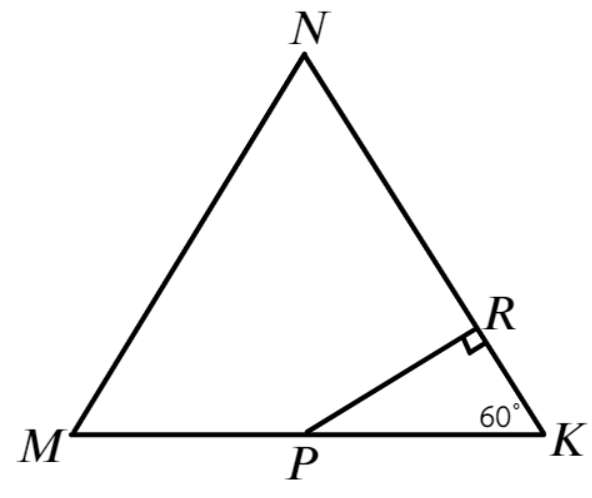
\includegraphics[scale=0.35]{g116.png}}
\end{figure}\\
Треугольник $MNK$ является равносторонним, значит все его углы равны $60^\circ.$ Тогда $\angle RPK=90^\circ-60^\circ=30^\circ.$ По теореме о катете, лежащем напротив угла в $30^\circ,$ имеем $KR=\frac{1}{2}PK=\frac{1}{4}MK=\cfrac{13}{4}.$\\
